\section{Estudios Térmicos}
\label{Ap:Estudio_termico}


\begin{figure}[h!]
            \centering
            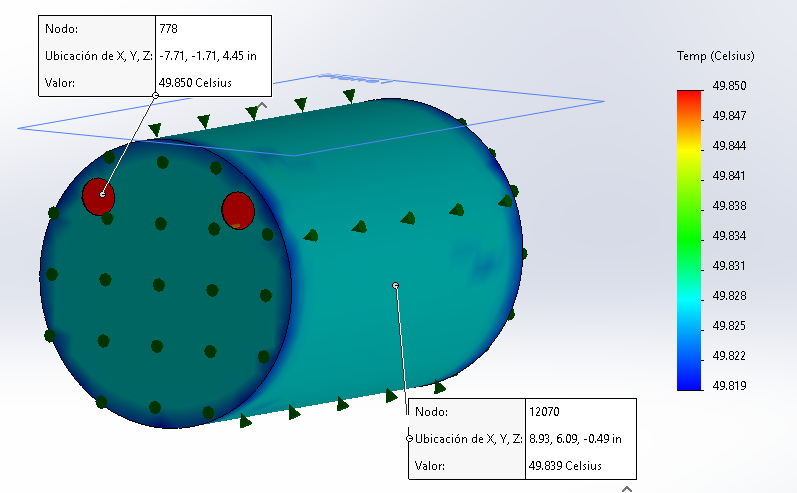
\includegraphics[scale=0.4]{images/Capitulo 4/s5/Contenedor/Est_Termicos/termicosf_3.png}
            \caption{Estudio térmico del contenedor}
            \label{fg:Estermico}
     \end{figure}

Lo que se puede observar aquí es que el calor pasa casi en su totalidad a la cara externa ya que se encuentra a .011 grados de la temperatura interna, lo que generará grandes pérdidas de calor. En un proceso de análisis el equipo se percató que este comportamiento podría representar un riesgo para quien manipule el dispositivo, puesto que si el usuario llega a tocar la parte externa, podría quemarse.

        \begin{figure}[h!]
            \centering
            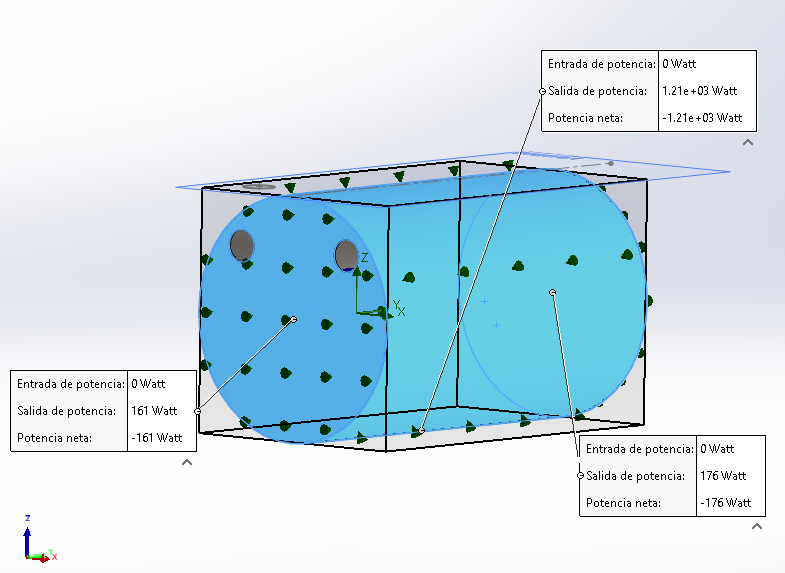
\includegraphics[scale=0.4]{images/Capitulo 4/s5/Contenedor/Est_Termicos/Potenciamod_3.png}
            \caption{Salida de potencia del modelo}
            \label{fg:Psf}
        \end{figure} \newpage

          \begin{figure}[h!]
            \centering
            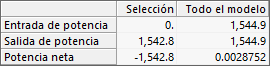
\includegraphics[scale=0.8]{images/Capitulo 4/s5/Contenedor/Potencia_total_modelo.png}
            \caption{Salida de Potencia total del modelo}
            \label{fg:Ptm}
        \end{figure}
        
Como se mencionó previamente, al pasar casi todo el calor a la cara externa del contenedor presentándose una potencia de salida de 1.544k W (Figura \ref{fg:Ptm}), lo que representa una gran pérdida de calor.

Tratando de contrarrestar este comportamiento que no es deseable para el funcionamiento del compostador se propone cubrir el contenedor un material aislante, en este caso se plantea utilizar fibra de vidrio, realizando la simulación recubriendo las paredes externas con este nuevo material (Figura \ref{fg:ETFV}).

    \begin{figure}[h!]
            \centering
            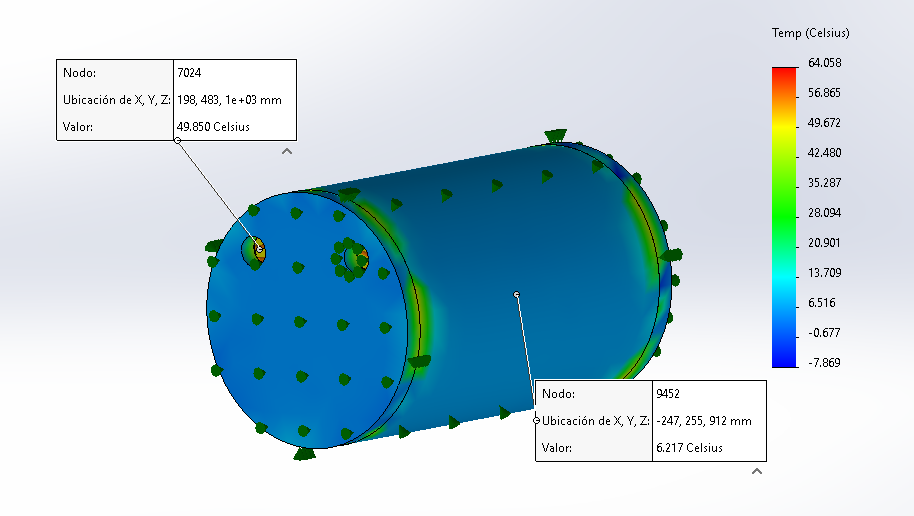
\includegraphics[scale=0.4]{images/Capitulo 4/s5/Contenedor/Est_Termicos/termico3_fibra.png}
            \caption{Estudio térmico con fibra de vidrio}
            \label{fg:ETFV}
        \end{figure}
Como se puede observar, los resultados mejoraron considerablemente, puesto que las caras externas se encuentras 3.217 grados por encima de la temperatura ambiental propuesta (3°C). Lo que permite mantener el calor al interior del contenedor, y en caso de que el usuario llegue a tocarlo, no se queme.

Estos resultados son coherentes ya que la conductividad térmica del acero corresponde a 51.9 W/mK y la conductividad de la fibra es de tan solo 0.04 W/mK, 1297.5 veces más pequeña que la conductividad del acero.

Y esto se puede observar en la potencia de salida, presentando los siguientes resultados (Figura \ref{fg:PmFV}).

  \begin{figure}[h]
            \centering
            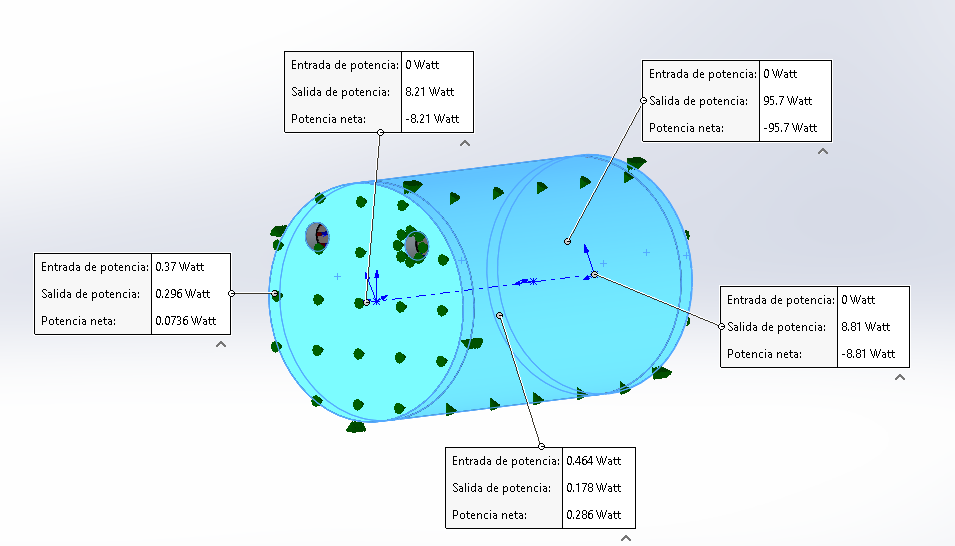
\includegraphics[scale=0.4]{images/Capitulo 4/s5/Contenedor/Est_Termicos/Potenciamod_3_fibra.png}
            \caption{Salida de Potencia con fibra de vidrio}
            \label{fg:PmFV}
    \end{figure}\newpage
        
        \begin{figure}[h]
            \centering
            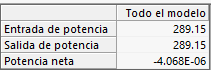
\includegraphics[scale=0.9]{images/Capitulo 4/s5/Contenedor/Est_Termicos/Potencia_fibra3.png}
            \caption{Salida de potencia total con fibra de vidrio}
            \label{fg:PTFV}
        \end{figure}
        
Como se puede apreciar en los resultados obtenidos con la potencia de salida total del modelo con fibra de vidrio (Figura \ref{fg:PTFV}) , es cinco veces menor en comparación a la salida de potencia total del modelo sin aislante térmico, lo que permite observar una reducción significativa del calor transmitido.

    Como se puede observar, los resultados obtenidos son bastante cercanos a los presentados teóricamente por otro lado, considerar la fibra de vidrio, puede beneficiar en gran manera el funcionamiento del circuito, ya que como se observó reduce la pérdida de calor, lo que en consecuencia evitaría el estar encendiendo continuamente las resistencias que calentarán el interior del contenedor, alargando así su vida útil y reduciendo de igual manera la energía consumida durante su funcionamiento.

Por otro lado, es bien sabido que la temperatura en la Ciudad de México cambia constantemente a lo largo del año, por lo que se propuso efectuar las simulaciones considerando una temperatura promedio de 16°C de acuerdo con datos del INEGI \cite{TempINEGI} y otra de 31.6°C siendo la temperatura más alta del año 2022 registrada en la ciudad de México de acuerdo a datos de la Secretaría de  Gestión Integral de Riesgos y Protección Civil (SGIRPC) \cite{Temp31}. Cabe señalar que la temperatura de 3°C se propuso debido a que se tiene pensado que la gran mayoría de pruebas se realizarán en épocas de días fríos del siguiente semestre, por lo que resultaba de interés observar el comportamiento del contenedor en un escenario similar. \newpage

Para 16°C sin aislante térmico, se obtuvieron los siguientes resultados:

\begin{figure}[h!]
            \centering
            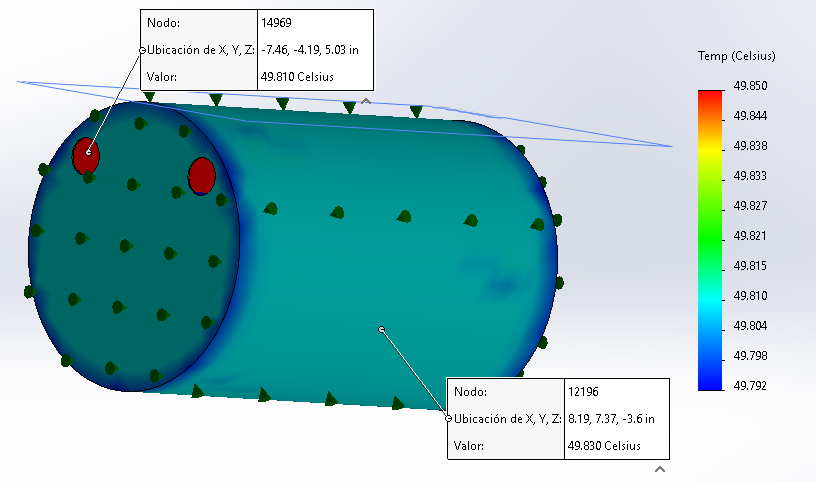
\includegraphics[scale=0.5]{images/Capitulo 4/s5/Contenedor/Est_Termicos/termicosf_16.png}
            \caption{Estudio térmico para una temperatura de 16°C}
            \label{fg:termico16}
        \end{figure}

        \begin{figure}[h!]
            \centering
            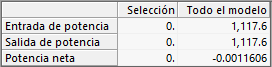
\includegraphics[scale=0.9]{images/Capitulo 4/s5/Contenedor/Est_Termicos/Potenciasf_16.png}
            \caption{Salida de potencia temperatura de 16°C}
            \label{fg:Potencia16}
        \end{figure}

Para 16°C con aislante térmico (fibra de vidrio), se obtuvieron los siguientes resultados:

\begin{figure}[h!]
            \centering
            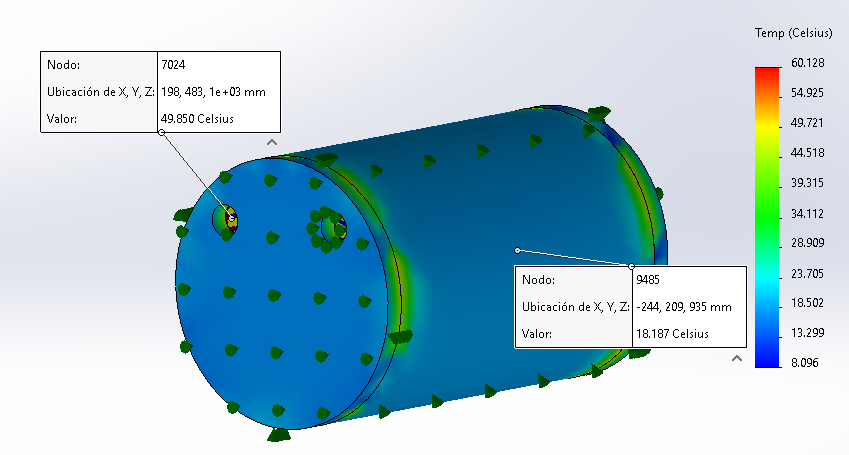
\includegraphics[scale=0.5]{images/Capitulo 4/s5/Contenedor/Est_Termicos/termico16_fibra.png}
            \caption{Estudio térmico para una temperatura de 16°C}
            \label{fg:termico16_fibra}
        \end{figure}

        \begin{figure}[h!]
            \centering
            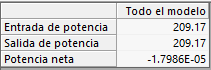
\includegraphics[scale=0.9]{images/Capitulo 4/s5/Contenedor/Est_Termicos/Potencia_fibra16.png}
            \caption{Salida de potencia temperatura de 16°C}
            \label{fg:Potencia16_fibra}
        \end{figure}

Para 31.6°C sin aislante térmico, se obtuvieron los siguientes resultados:

\begin{figure}[h!]
            \centering
            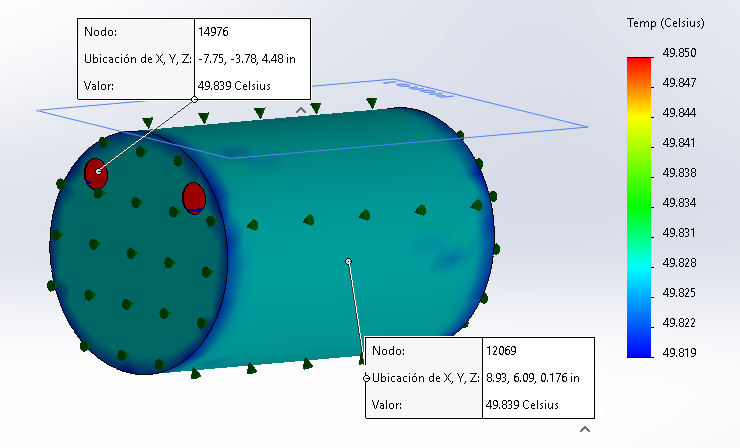
\includegraphics[scale=0.5]{images/Capitulo 4/s5/Contenedor/Est_Termicos/termicosf_31.6.png}
            \caption{Estudio térmico para una temperatura de 31.6°C}
            \label{fg:termico31}
        \end{figure}

        \begin{figure}[h!]
            \centering
            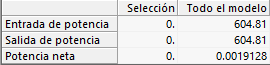
\includegraphics[scale=0.9]{images/Capitulo 4/s5/Contenedor/Est_Termicos/Ptenciasf_31.6.png}
            \caption{Salida de potencia temperatura de 31.6°C}
            \label{fg:Potencia31}
        \end{figure}

Para 31.6°C con aislante térmico (fibra de vidrio), se obtuvieron los siguientes resultados:

\begin{figure}[h!]
            \centering
            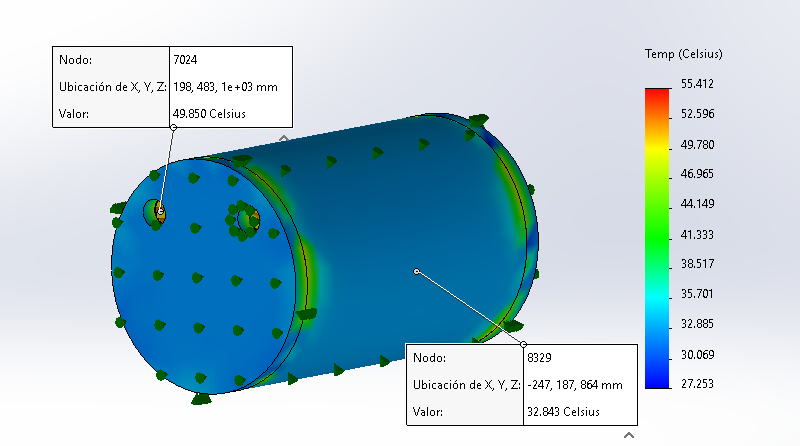
\includegraphics[scale=0.5]{images/Capitulo 4/s5/Contenedor/Est_Termicos/termico31_fibra.png}
            \caption{Estudio térmico para una temperatura de 31.6°C con aislante térmico}
            \label{fg:termico31_fibra}
        \end{figure}

        \begin{figure}[h!]
            \centering
            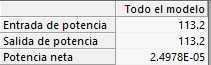
\includegraphics[scale=0.9]{images/Capitulo 4/s5/Contenedor/Est_Termicos/Potencia_fibra31.png}
            \caption{Salida de potencia temperatura de 31.6°C con aislante térmico}
            \label{fg:Potencia31_fibra}
        \end{figure}